\RequirePackage[l2tabu, orthodox]{nag} %Package complains about uses of old functions, make sure you write modern latex
\documentclass[letterpaper,12pt,twoside,openright]{report} %twoside an openright make the doucment look like a "real textbook" style formatting
\usepackage[english,canadian]{babel}
\usepackage{amsmath} %AMS Math Package
\usepackage{amssymb} %AMS Math Symbols
\usepackage[all,warning]{onlyamsmath}%Warn about non-ams math useage, suggest improvements
\usepackage[letterpaper,twoside,top=3.8cm,bottom=2.5cm,inner=2.5cm,outer=3.8cm]{geometry} %Sets up basic page dimensions
\usepackage[tracking=true,kerning=true,expansion=true,spacing=true]{microtype} %makes type look better
\microtypecontext{spacing=nonfrench}
\usepackage{booktabs} %makes tables look better with nicer borders
\usepackage{siunitx} %provides standard printing for SI units
\usepackage[breaklinks,hidelinks]{hyperref} %Provides clickable links
\usepackage[capitalize,noabbrev]{cleveref} %Allows use of \cref, which knows what kind of ref you're making, so you don't have to write EQN and such
\usepackage{ifpdf} %Conditions for if pdftex is running
\usepackage[T1]{fontenc} %upgrades font encodings
\usepackage[utf8]{inputenc}%Tells latex the file is saved as UTF-8 (make sure it is!)
\usepackage{lmodern} %improved version of computer modern font
\usepackage{multirow} %Allows for mulirow a.k.a. grouped cells in tables
\usepackage{fixltx2e} %Fixings bugs in latex2e that aren't fixed due to breaking backwards compatability
\usepackage{upgreek} %Provides upright (non italic) greek fonts
\usepackage{gensymb} %Provides  \de­gree, \cel­sius, \pert­hou­sand, \mi­cro and \ohm amongst others
\usepackage{textcomp}
\usepackage{textgreek} %Provides \textbeta and similar greek letters in text mode
%\usepackage[section]{placeins} %Fixes placement of figures so they don't cross section boundaries
\usepackage[section,subsection,subsubsection]{extraplaceins} %Modified version of placeins which works at section, subsection and subsubsection
\usepackage{verbatim}%Fixes bugs in \verbatim, and provides \begin{comment} and \verbatiminput for including files
\usepackage{syntonly}%Provides syntax-only latex runs, useful for when the document starts getting big!
\usepackage{csquotes}
\usepackage{float} %Fixes up floats (figures) and provides the H placement modifier (place the float RIGHT HERE). with great power...
%\usepackage[style=numeric-comp,backend=biber,sorting=none,backref=true,maxnames=99,alldates=iso8601]{biblatex} %Sets up the referencing system, standard numeric ordering, prints the page numbers refereced as a back reference, prints all names, makes dates iso dates
\usepackage[style=numeric-comp,backend=biber,sorting=none,backref=true,maxnames=99,alldates=iso8601,refsection=chapter]{biblatex}
\addbibresource{library.bib} %This is how you add your bib files
\usepackage[english]{isodate}%Convert any date formats to ISO style
\usepackage{listing}%Package for listing sourcecode with syntax highlighting
\usepackage{ellipsis}%Fix \ldots and similar commands, bugs with spacing and such
\usepackage{graphicx} %Standard graphics spackage
\setkeys{Gin}{width=0.75\textwidth} %Sets default width of \includegraphics{}
\usepackage{lastpage} %Used to count the number of pages for the descriptive note
\usepackage{nomencl} %Used to generate the Abbreviations page
\usepackage[raggedright]{titlesec} %This fixes hypenation in long chapter/section titles

\pdfminorversion=5 %This sets the PDF versions allowing better compression
\pdfobjcompresslevel=3
\pdfcompresslevel=9

\usepackage{subcaption} %The standard method to do figures with a), b) and such
\usepackage{fancyhdr} %Package for changing header/footer
\usepackage{lineno} %Allows labeling of line numbers throughout document
\usepackage{makeidx} %For generating index files
\usepackage{lipsum} %Prints junk text with \lipsum
\usepackage{setspace} %Provides \doublespacing command
\usepackage{todonotes} %Provides \todo{something} which puts labels in magin and \missingfigure{something} to put in placeholder figures

\widowpenalty=300 %Prevent widows (single sentences at end of page)
\clubpenalty=300 %Prevent orphans (single sentences on empty pages)
\doublespacing %Uncomment to turn on double spacing
%\onehalfspacing %Double spacing is crazy large, don't do it.
%\linenumbers %Uncomment to turn on line numbers
%\syntaxonly %Uncomment to only check compile for syntax PRODUCES NO OUTPUT
\setlength{\headheight}{15pt} %Fixes header height

\hypersetup{
    unicode=true,
    pdftoolbar=true,
    pdfmenubar=true,
    pdffitwindow=false,
    pdfstartview={FitV},
    pdftitle={Integrating sphere-based spectrally constrained total diffuse reflectance for in vivo quantification of hemoglobin in skin},
    pdfauthor={Diana L. Glennie},
    pdfsubject={Subject},
    pdfkeywords={keyword1} {key2} {key3},
    pdfnewwindow=true,
    colorlinks=false,
    linkcolor=red,
    citecolor=green,
    filecolor=magenta,
    urlcolor=cyan
}
%\graphicspath{{graphics/}} %Uncomment if you want to hide all figure files in a graphics/ subdirectory

\title{Integrating sphere-based spectrally constrained total diffuse reflectance for in vivo quantification of hemoglobin in skin}
\author{Diana L. Glennie}
\date{\today}

%This stuff is used to generate a nomenclature section
\makeindex
\renewcommand{\nomname}{List of Abbreviations and Symbols}
\renewcommand{\nomlabel}[1]{\textbf{#1}}
\makenomenclature
\raggedbottom
\begin{document}

\begin{titlepage} %Half-title page for McMaster Formatting, Max 60 Characters
    \thispagestyle{empty}
    \topskip0pt
    \vspace*{\fill}
    \begin{center}{\Large
    \uppercase{In vivo quantification of hemoglobin in skin}}
    \end{center}
    \vspace*{\fill}
    \setcounter{page}{0} %This page needs to be "unnumbered" so we give it number zero
\end{titlepage}

% % % % % % % % % % % % % % % % % % % % % % % % % % % % % % % % % % % % % %
\begin{titlepage} %Titlepage
\thispagestyle{empty}
\pagenumbering{roman}
\centering
\vspace*{\fill} %This makes text vertically centered
{\Large \uppercase{Integrating sphere-based spectrally constrained total diffuse reflectance for in vivo quantification of hemoglobin in skin}\\
\vfill
By DIANA L.\ GLENNIE, B.\ SC., M.\ SC.\\}
\vfill
A Thesis Submitted to the School of Graduate Studies in Partial Fulfilment of
the Requirements for the Degree Doctor of Philosophy
\vfill%This pushes copyright to the bottom
McMaster University \textcopyright{} Copyright by Diana L.\ Glennie, November 2014
\end{titlepage}
% % % % % % % % % % % % % % % % % % % % % % % % % % % % % % % % % % % % % %
{\noindent McMaster University DOCTOR OF PHILOSOPHY (2014) Hamilton, Ontario (Medical Physics)\\
TITLE: Integrating sphere-based spectrally constrained total diffuse reflectance for in vivo quantification of hemoglobin in skin\\
AUTHOR: Diana L. Glennie, B.Sc., M. Sc. (McMaster University)\\
SUPERVISOR: Professor Thomas J. Farrell\\
NUMBER OF PAGES: ix,~\pageref{LastPage}}
% % % % % % % % % % % % % % % % % % % % % % % % % % % % % % % % % % % % % %
    \begin{abstract}
        \thispagestyle{plain}
        \setcounter{page}{3}
            An abstract of not more than 300 words must be included and will indicate the major emphasis of the thesis, new discoveries, and its contribution to knowledge. The style of abstract varies somewhat from discipline to discipline; the student should follow an appropriate style.
    \end{abstract}

    \renewcommand{\abstractname}{Acknowledgements}
    \begin{abstract} \setcounter{page}{4} \thispagestyle{plain}
        This is where I get all mushy and thank the people who've helped me get to where I am today.
    \end{abstract}
    
    \setcounter{secnumdepth}{3} %Make TOC include subsubsections
    \tableofcontents %Prints table of contents
    {\listoffigures \let\cleardoublepage\clearpage %This fixes up an extra blank page
    \printnomenclature} %Print glossary/nomenclature/abbreviations

    \renewcommand{\abstractname}{Declaration of Academic Achievement}
    \begin{abstract} \thispagestyle{plain} \setcounter{page}{9} %This page number needs to be manually set properly after the tableofcontents is generated
        The work presented here is the result of research performed by myself during the years 2009--2014. Results that have substantial contributions from other authors are clearly prefaced and the contributions of those authors are indicated.
    \end{abstract}
    
    %\listoftodos %Uncomment this to generate a list of todos (useful for keeping track of things)
    \pagenumbering{arabic} %Reset page numbering

%Fix all the header/footer according to McMaster Requirements
    \pagestyle{fancy}
    \fancyhead{}
    \fancyfoot{}
    \fancyhead[RE,LO]{McMaster University --- Medical Physics}
    \fancyhead[LE,RO]{PhD Thesis --- Diana L. Glennie}
    \fancyfoot[CE,CO]{\thepage}

% % % % % % % % % % % % % % % % % % % % % % % % % % % % % % % % % % % % % %
%Thesis starts here

%For large LaTeX documents, it is best practice to separate the material into smaller files so that it is easier to handle, use \include to insert each file into the overall document

\chapter{Introduction}
\section{Motivation}
The ability to measure changes in the hemoglobin concentration in skin will enable more personalized patient care which, in turn, may lead to an increase in treatment success rates and a decrease in per-patient costs.

For example, in radiation therapy, a common side effect is a skin-reddening reaction known as erythema, or radiation dermatitis.\cite{McQuestion2006} Depending on the severity of the reaction, erythema can be quite painful and may even prevent the completion of the radiation treatment schedule, thereby reducing the overall treatment efficacy. Unfortunately, since it is a deterministic effect,\cite{Hall2000} with a varying threshold dose and a spectrum of reactions, erythema is impossible to reliably predict in advance. Instead, patients’ responses are monitored by the therapy team over the course of treatment. The current method for monitoring erythema is by visual assessment (VA). VA uses a pre-determined scale to classify the current condition of the skin. If there are too few divisions on the scale (four or less), there is not a sufficient amount of information regarding the patient’s progress from the erythema stage to the next stage of moist desquamation. If there are more than four divisions on the scale, it is difficult to eliminate, or even minimize, the inter- and intra-observer variation, making the results unreliable at best, and preventing any comparison between patients. The implementation of an objective method for measuring skin redness would allow for the treatment team to better manage the reaction, thus improving the treatment’s success rate and the patient’s quality of life.

Another application of a quantitative system for monitoring the hemoglobin concentration in skin is in the field of plastic surgery. Prior to incision, lidocaine (an anesthetic) and epinephrine (a hormone used for vasodilation) are commonly used to numb the surgical region and reduce bleeding during surgery. The commonly cited time to maximal effect of epinephrine is 7-10 minutes, but this time interval was approximated with a porcine model\cite{Larrabee1987} using laser Doppler flowmetry\cite{Swain1989} and was never confirmed with human trials and quantitative measurements.

\section{Light-tissue interactions}
The propagation of light in tissue can be described by three main interactions:\cite{Niemz2007}
\begin{enumerate}
	\item Reflection (and refraction)
	\item Absorption
	\item Scattering
\end{enumerate}

Reflection and refraction occur at the boundary between two materials with different indices of refraction, such as between air and tissue. Neither process can occur if the two materials have equal indices of refraction. For a smooth surface, the light that is reflected at the boundary obeys the law of specular reflection which states that the angle of reflection of a ray of light is equal to the angle of incidence.\cite{Knight2013} Light that is transmitted past the boundary refracts toward the normal as described by Snell's law,

\begin{equation}
n_1 \sin \theta_1 = n_2 \sin \theta_2
\end{equation}

\noindent where $n_1$ and $n_2$ are the indices of refraction of the two materials, $\theta_1$ is the angle of incidence, and $\theta_2$ is the angle of refraction.

The amount of light that undergoes either of these two processes can be predicted using Fresnel's equations which require the relative index of refraction ($n_2 / n_1$) and the angle of incidence ($\theta_1$) as their input parameters.\cite{Pedrotti1993} It should be noted that, while most applications approximate the indices of refraction as constants, there is a small wavelength dependence present that should be considered for large wavelength ranges.\cite{Knight2013}

While inside a material, light can either be absorbed or scattered. The probabilities of these two occurrences are based on the optical properties of the material. When an absorption event occurs, the light energy is transferred to a bound electron, elevating it to an excited state.\cite{Jacques2004} Atoms or molecules with excited electronic states can ``discharge'' this energy either through radiative processes such as fluorescence or phosphorescence or, more commonly, through non-radiative processes like vibration. The probability of absorption occurring within an infinitesimal distance $ds$ is $\mu_ads$, where $\mu_a [mm^{-1}]$ is the absorption coefficient. The inverse of the absorption coefficient represents the distance between absorption events. In the case of (elastic) scattering, the energy is absorbed by a free electron that causes acceleration and the emission of a secondary photon with the same frequency.\cite{Jacques2004} The probability of scattering occurring within an infinitesimal distance $ds$ is $\mu_sds$, where $\mu_s [mm^{-1}]$ is the scattering coefficient. The inverse of the scattering coefficient represents the distance between scattering events.

Elastic scattering is isotropic in nature. That is, it is equally probable for the photon to be emitted in any direction. In a homogeneous medium, all directions except the initial photon direction cancel. However, in a medium with many small, suspended particles, another direction may dominate. This can be accounted for with an anisotropy factor ($g$) that is equal to the expectation value (also the average value) of the cosine of the scattering angle. An anisotropy factor of $0$ represents isotropic scattering while a factor of $1$ represents forward scattering. To account for this directionality when modeling light transport in tissue, a reduced scattering coefficient is commonly defined as $\mu_s'=(1-g)\mu_s$ such that its inverse is the distance between isotropic scattering events that produces the same results as the anisotropic scattering.\cite{Gratton2004}

Another helpful quantity is the total reduced attenuation coefficient, $\mu_t'=\mu_a + \mu_s'$ which, when multiplied by an infinitesimal distance, represents the probability of any interaction occuring within that infinitesimal distance. Its inverse is specially termed the ``mean free path'' and represents the average distance between interactions.\cite{Farrell2003}

\section{Modeling of light transport in turbid material}

\subsection{Radiation transport equation and diffusion theory}
The radiation transport equation (RTE), also known as the Boltzmann equation, describes the transfer of neutron particles (in this case, energy in the form of photons) within an infinitesimal volume as a function of time.\cite{Duderstadt1976} It is often expressed as a change in the time- and space-resolved energy radiance, $L(\mathbf{r},\mathbf{\Omega},t)$ with respect to time. This quantity can be determined by investigating the mechanism by which the energy radiance can be gained and lost from the volume in question. When considering the steady-state condition, there is no net change in the energy radiance and the gain terms equal the loss terms.

\noindent The gain mechanisms are:
\begin{enumerate}
	\item Any photon sources within the volume, $ S(\mathbf{r},\mathbf{\Omega}) $
	\item Photons already within the volume that scatter into the direction of interest,  $\int_{4\pi} L(\mathbf{r},\mathbf{\Omega}) \mu_s(\mathbf{r},\mathbf{\Omega}' \rightarrow \mathbf{\Omega}) d \mathbf{\Omega'} $
	\item Photons that enter into the volume along the direction of interest
\end{enumerate}

\noindent Loss mechanisms include:
\begin{enumerate}
	\item Photons that are absorbed within the volume, $ \mu_a L(\mathbf{r},\mathbf{\Omega}) $
	\item Photons that scatter out of the volume, $ \mu_s L(\mathbf{r},\mathbf{\Omega}) $
	\item Photons that exit the volume
\end{enumerate}

\noindent A single convection term can be used to account for the photons entering and exiting the volume, $-\mathbf{\Omega}\cdot\nabla L(\mathbf{r},\mathbf{\Omega})$. The combination of all of the terms results in the following equation for the steady-state RTE,\cite{Farrell2003}

\begin{equation}
\label{eq:rte}
\mathbf{\Omega}\cdot\nabla L(\mathbf{r},\mathbf{\Omega}) + (\mu_a + \mu_s) L(\mathbf{r},\mathbf{\Omega}) - \int_{4\pi} L(\mathbf{r},\mathbf{\Omega}) \mu_s(\mathbf{r},\mathbf{\Omega}' \rightarrow \mathbf{\Omega}) d \mathbf{\Omega'} - S(\mathbf{r},\mathbf{\Omega}) = 0
\end{equation}

Solutions to the above equation may be found via intense numerical methods, but they are extremely computationally expensive. As such, a simpler approach is often employed, in which approximations are made that simplify the RTE into a solution-friendly form. In the case of light transport in tissue, the diffusion approximation simplifies the above equation into a single differential equation.
Diffusion theory requires the radiance to be isotropic. This condition is generally met in a semi-infinite medium at a point greater than 1 mfp away from the source or boundaries\cite{Jacques2004} and when $ \mu_a < 0.1\mu_s'$.\cite{Wilson2008} In other words, when the probability of scattering is much greater than the probability of absorption, the direction of the photons is mostly randomized after only a few scattering events, or 1 mfp. The result of these approximations is the diffusion equation as follows,

\begin{equation}
\label{eq:diffeq}
\nabla^2 \cdot \Phi(\mathbf{r}) - \frac{\mu_a}{D}\Phi(\mathbf{r}) = S(\mathbf{r})
\end{equation}

Where $\Phi(\mathbf{r})$ is the energy fluence rate (the integral of the energy radiance over all angles), $D$ is the diffusion constant, $(3\mu_t')^{-1}$, and $S(\mathbf{r})$ is the source term.

The diffusion equation can be solved analytically by applying a set of boundary conditions. In the case of tissue optics, the most common boundary conditions have been developed to account for the mismatch in the index of refraction between the tissue and the air, and the resulting Fresnel reflections from the interior surface of the tissue.

\subsection{Monte Carlo simulations}
\label{sec:mc}
Monte Carlo (MC) simulations offer a method of solving the steady-state RTE that is slightly less computationally expensive than traditional numerical methods. It is also useful for confirming solutions for approximations such as diffusion theory. Millions of photons are ``launched'' and their propagation through the medium is determined by the random sampling of probability distributions that represent the absorption and scattering conditions of the medium. The basic principles of MC simulations have been thoroughly covered by Prahl \emph{et al.}\cite{Prahl1989} and Wang \emph{et al.},\cite{Wang1995} so only two important variations are outlined here.

If a single simulation must be run several times with different sets of optical properties, it is useful to adapt the code into what has been termed mono (or “white”) MC.\cite{Kienle1996a,Alerstam2013} Under this simulation, photons are tracked through a homogeneous scattering, non-absorbing medium. There is no survival weighting in mono MC, so the photons' weights are never modified in the tissue and they are only killed when they scatter too many times (via Russian roulette) or they migrate too far from the region of interest. The total distance traveled by each photon (the pathlength, $s$) in the medium is tracked. When photons are finally scored, their weight is added to a bin for the corresponding total pathlength. The effect of absorption can be introduced after the simulation is complete by multiplying each bin by $\exp(-mua*s)$ and summing over all the bins.

When multiple processors are available on a computer, parallelization is an option for increasing the speed of the MC simulation. In parallel computing, single calculations are performed by each available processor in a computer and the results are collated at the end. Parallelization is only possible if all the calculations are independent of one another (i.e. the order doesn't matter). Since MC is based on stochastic processes, each photon can be treated separately. For example, in a computer with four processors, it is possible to track four photons simultaneously, recording their progress, and collect their results once terminated. This yields a MC simulation that would run four times faster than the original, serial code.

\section{In vivo measurements of tissue optical properties with diffuse reflectance}
\label{sec:diff_refl}
For the purposes of monitoring patient response, \emph{ex vivo} methods for determining tissue optical properties are obviously not appropriate. Therefore, this section will focus solely on a specific subset of available \emph{in vivo} methods – those that require steady-state conditions, as opposed to time resolved systems.

\subsection{Total diffuse reflectance}
\label{sec:total_diff_refl}
The total diffuse reflectance represents the fraction of incident light fluence remitted from the tissue across the entire surface (i.e. it is spatially integrated) at a single wavelength. It can be modelled with the diffusion approximation and is dependent only on the reduced albedo and the relative index of refraction.\cite{Kim2011} The index of refraction for skin has been accurately measured, and a value of 1.4 is typically used for incident light within the visible spectrum.\cite{Kienle1996a} With this information, the albedo of the tissue can be determined from the measured total diffuse reflectance. For a single total diffuse reflectance measurement, there is no way to determine the individual contributions from scattering and absorption. However, if the scattering and mean pathlength are assumed constant, a second measurement, where the absorption coefficient is known or can be approximated, will allow for the determination of the first absorption coefficient. This technique relies on the relationship between the total diffuse reflectance and the exponential of the absorption coefficient and the pathlength. The total diffuse reflectance is generally measured either with an integrating sphere (see Section~\ref{sec:is_theory}) or with an optical system, off-set from the normal to avoid collecting any specular reflectance.

\subsection{Spatially-resolved diffuse reflectance}
\label{sec:spat_diff_refl}
The spatially-resolved diffuse reflectance is the fraction of the incident light remitted at a set of radial distances from the incident light source. It can be collected in one of two ways: either with an imaging system\cite{Kienle1996b} or by detection fibers positioned at many (at least two) distances from the source fiber.\cite{Kim2011}

When the reflectance is captured with an imaging system, such as a digital camera, the radially-dependent reflectance curve can be constructed by binning pixel intensities at equal radial distances. This method provides more data points for the subsequent analysis. A weak point in this collection method is that, unless a hyperspectral camera is used, only the optical properties at a single wavelength (that of the incident laser source) can be determined.

When measuring reflectance with a fiber optic array, the optical properties can be determined for a range of wavelengths as a white light source and a spectrometer will allow for the resolution of this data. The source and detection fibers are usually bundled together in a single probe to maintain accurate and consistent positioning of the fibers. Several probes are used at greater distances to improve the signal-to-noise ratio(see Figure~\ref{fig:intro-srdr}).

\begin{figure}
	\centering 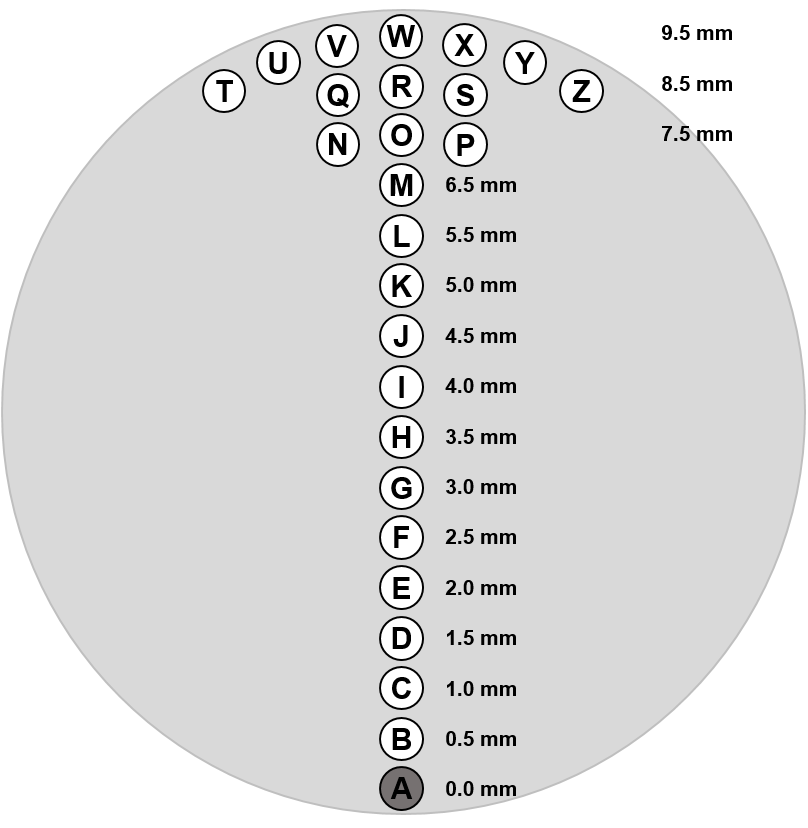
\includegraphics[width=0.5\textwidth]{figures/intro-srdr.png}
	\caption[Probe for spatially-resolved diffuse reflectance]{\label{fig:intro-srdr}A diagram representing the configuration of the optical fibers in the probe. Light enters through fiber “A” (dark grey) and is detected by additional fibers that are placed set distances away (white).}
\end{figure}

Both the absorption and reduced scattering coefficients can be determined from this collected data. One analysis method is to compare the obtained results to those from a single Monte Carlo simulation. In addition to applying the effect of absorption post-simulation (see Section~\ref{sec:mc}), it is also possible to scale the results for different scattering coefficients from a single reference scattering coefficient as follows,\cite{Kienle1996a}

\begin{equation}
	R(\rho) = \left(\frac{\mu_s'}{\mu_{sref}'}\right)^2 R_{ref}\left(\rho\frac{\mu_s'}{\mu_{sref}'}\right)
\end{equation}

\noindent where the ratio of the new reduced scattering coefficient to the reference reduced scattering coefficient acts as a scaling factor. A fitting algorithm will vary the optical properties and generate a reflectance curve from the MC data until the resulting chi-squared statistic between the measured data and the calculated data is minimized.

The data can also be fitted with a nonlinear equation for the spatially-resolved reflectance derived from diffusion theory. The absorption and reduced scattering coefficients would act as input parameters for the equation and those that resulted in the best fit (via a given fitting algorithm) would be the approximate values. When deriving this equation, the selection of the boundary conditions is integral in recovering reliable results. Farrell \emph{et al.}\cite{Farrell1992} used an ``extrapolated'' boundary condition and an negative image source to yield a fluence rate of zero at a new (extrapolated) boundary located above the actual tissue-air interface. The height of the image source and the boundary are dependent on the tissue optical properties. Using this set of approximations and boundary conditions, the recovered values for the absorption and reduced scattering coefficients agreed with the true values within 10\%.

%\begin{equation}
	%R(r) = \frac{1}{4\pi}\left[z_0 \left(\mu_{eff} + \frac{1}{\rho_1}\right) \frac{e^{-\mu_{eff}\rho_1}}{\rho_1^2} + \left(z_0 + 2z_b\right) \left(\mu_{eff} + \frac{1}{\rho_2}\right) \frac{e^{-\mu_{eff}\rho_2}}{\rho_2^2}  \right]
%\end{equation}

\subsection{Spectrally-constrained diffuse reflectance}
\label{spec_diff_refl}
Due to advances in technology, a recently popular method employs a single source-detector pair instead of a spatially-resolved array of detector fibers. In this approach, a broad beam light source is used instead of a single wavelength light source, and the collected signal is resolved into a reflectance measurement at each wavelength. However, this reflectance spectrum is not sufficient to determine the tissue optical properties. Generally, a forward model of the diffusion theory is derived and fit to the obtained reflectance spectrum. Such a model requires both the absorption and reduced scattering coefficient spectra, which can be approximated.

The absorption coefficient is estimated to be the sum of the individual chromophore concentrations $c_i$, multiplied by their respective extinction coefficient spectra $\varepsilon_i(\lambda)$, as follows,

\begin{equation}
\mu_a(\lambda) = \sum_i c_i \varepsilon_i(\lambda)
\end{equation}

The extinction coefficient is the absorption coefficient per molar ($mol/L$) for the medium. These spectra for the majority of chromophores found in human skin (see Section~\ref{sec:skin}) have been well characterized and the chromophore concentrations are included as fitting parameters in the forward model. It is important to include only those chromophores that contribute significantly to the overall absorption within the wavelength range of interest. Including insignificant chromophores will add too many variables to the fitting equation while omitting significant chromophores will yield inaccurate results.

The reduced scattering coefficient for human skin has been well-characterized and follows a wavelength-dependent power law,\cite{Doornbos1999}

\begin{equation}
\mu_s'(\lambda) = a\lambda^{-b}
\end{equation}

As a result, the scaling factor ($a$) and the exponential ($b$) can be included as fitting parameters in the forward model.

\subsection{Commercially available systems}
Currently available commercial systems that measure diffuse reflectance are primarily used in dermatological applications. As such, their focus is on measuring the skin color which is directly related to the concentrations of the chromophores found in skin.

Two such systems are the DSM II Skin ColorMeter (Cortex Technology, Hadsun, Denmark) and the Mexameter\textregistered MX 18 (Courage+Khazaka electronic GmbH, Cologne, Germany). The DSM II Skin ColoMeter employs a plastic probe with focusing optics to shine a white LED onto the skin surface. The reflected light is then focused back onto multispectral detectors within the probe. The detector processes the reflected signal into one of the many color systems (RBG, CMYK, or L*a*b*) or an undefined erythema index. The Mexameter uses three distinct wavelengths (568 nm, 660 nm, and 870 nm) emitted by a 16 LED array onto the skin within a probe head that is placed on the skin surface. The red and near-infrared (NIR) wavelengths are used to determine a melanin index, and the green and red wavelengths are used to determine the erythema index .\cite{Clarys2000} Both systems relies on calibration measurements performed on black and white reflectance standards (provided).

Prices for either system could not be determined, but a recent competitor, the Derma Spectrometer (MIC Global, London, United Kingdom) (no longer for sale) was selling for \$6000 in early 2014.

\section{Integrating sphere theory}
\label{sec:is_theory}
An integrating sphere is a light delivery and/or collection device. As its name suggests, it is made from a sphere with several ``ports'' cut out of the surface through which light can enter or exit. A typical sphere is shown in Figure~\ref{fig:intro-is_sample}. The inner surface of the sphere is covered with a highly diffuse reflective coating to create what is known as a Lambertian surface. When used as a light delivery device, the light emitted from the irradiation port is uniformly distributed and is isotropic in direction. When used as a measurement device, it is capable of capturing all of the light emitted from the sample area directly below the measurement port. Together, these illumination and measurement qualities make integrating spheres ideal for measuring the total diffuse reflectance (spectra).

\begin{figure}
	\centering 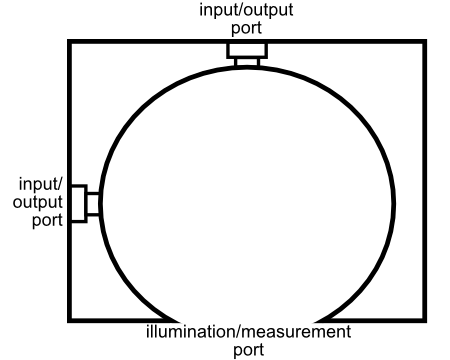
\includegraphics[width=0.5\textwidth]{figures/intro-is_sample.png}
	\caption[Sample integrating sphere diagram]{\label{fig:intro-is_sample}A diagram displaying a common geometry for an integrating sphere. There are two ports for delivering and collecting the light and one port for measuring the reflectance from a sample.}
\end{figure}

\subsection{Relative reflectance and sphere throughput}
The total diffuse reflectance is a relative (as opposed to absolute) reflectance measurement. As such, it requires a characterized reflectance sample known as a reference standard. Measurements performed with the sample of interest are compared (usually as a ratio) to measurements performed with the reference standard. To ensure accurate reflectance measurements, it is important to maintain a consistent throughput, or efficiency within the sphere between the sample and the standard measurements.\cite{Hanssen2002}

The throughput or efficiency of an integrating sphere is the best way of characterizing its performance. It can either be empirically determined or approximated by the following equation,

\begin{equation}
\tau = f_d \frac{\rho_w}{1-\bar{\rho}_w}
\end{equation}

\noindent where $f_d$ is the exchange factor which is equal to the ratio of the total surface area of all the ports to the surface area of the sphere, $\rho_w$ is the actual reflectance of the sphere wall material, and $\bar{\rho}_w$ is the average sphere wall reflectance accounting for the reflectances at the ports.

When the integrating sphere is sufficiently large, a change in the reflectance at one of the ports has a proportionately small effect on the sphere's throughput. Unfortunately, large spheres are not only expensive, but often impractical. For smaller spheres, changes in the sphere throughput between the sample and the reference standard cause what are known as Single Beam Substitution Errors (SBSE) in the total diffuse reflectance measurement.

If the sphere is sufficiently large to allow for an additional ``dummy'' port, a second measurement can be performed to account for SBSE, as shown in Figure~\ref{fig:intro-is_compar}.\cite{Labspherec} The geometry for the first measurement positions the sample directly opposite the light source and the reference standard at the dummy port. This is the primary reflectance measurement. The geometry for the second measurement positions the reference standard directly opposite the light source and the sample at the dummy port. This represents the background correction factor. Under this experimental design, the sphere throughputs and average reflectances are equal for the two measurements.

\begin{figure}
	\centering 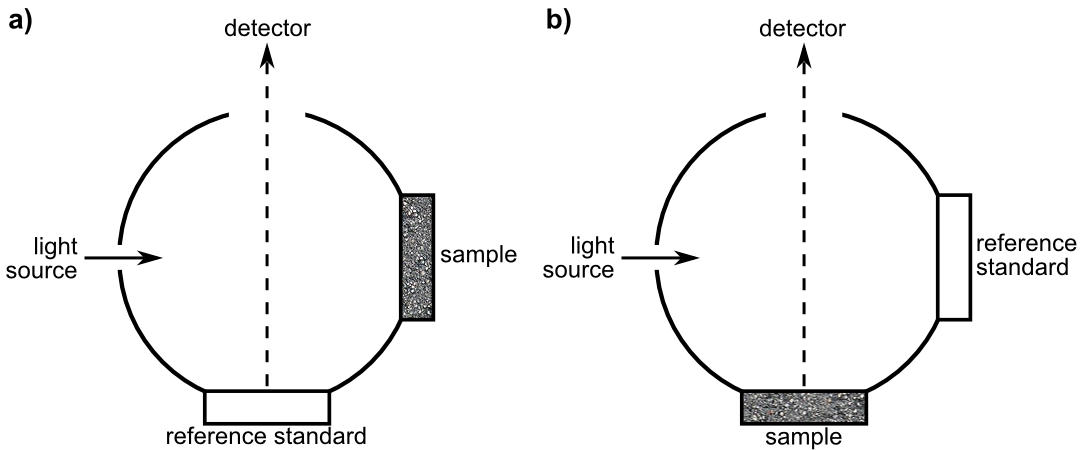
\includegraphics[width=1.0\textwidth]{figures/intro-is_compar.png}
	\caption[The comparison method for measuring sample reflectance]{\label{fig:intro-is_compar}To ensure a constant throughput in the sphere between sample and reference measurements, a dummy port can be added to sufficiently large spheres.}
\end{figure}

If the sphere is too small to permit a second port, the SBSE must be corrected mathematically or empirically. Of these two options, the empirically approach is preferred as a mathematical solution would be extremely complex and only accurate if precise values for parameters such as port fractions and reflectances were provided. For a given sphere, measurements are performed on a set of characterized reflectance standards covering the range of reflectances expected from the samples. By comparing the observed reflectances to the expected ones, a correction factor equation or a lookup table can be produced. REFERENCE TO PAPER \#1?

\subsection{Integrating sphere design}
When creating a new integrating sphere, there are several major designs considerations that must be optimized to minimize measurement error. The first of such options is the sphere size which cannot be determined until the total surface area of all of the ports is determined. Ports intended for coupling with optical fibers will have a set surface area while the size of the detection/illumination port(s) will depend on the use of the sphere. Once the total surface area of the ports has been determined, the sphere size can be calculated based on the rule of thumb that the resulting exchange factor be less than 5\%.\cite{Labsphereb} Spheres that exceed this ratio no longer display some of the desired characteristics such as the isotropy of the light within the sphere.

The next consideration is the material of the sphere, or the sphere's internal coating. Spheres can be created from a highly reflective material such as Spectralon, or they can be produced with a standard plastic material and subsequently coating on the inside with a highly reflective paint, such as barium sulfate. In either case, it is extremely important that the interior surface of the sphere have as high a reflectance as possible, ideally greater than 94\%. This material should also be matte or diffuse in nature, not glossy to produce the desired scattering that creates the isotropic illumination.

The final consideration for the integrating sphere would be the geometry of the ports. With few exceptions, it is important for light from the input port to not be directly incident on the output port. To accomplish this, the numerical aperture of the optical fibers connected to the ports and the overall sphere geometry should be considered. If physical positioning of the ports cannot accomplish this task,  wall projections into the center of the sphere, known as baffles, can be added. Baffles are not ideal for smaller spheres as they introduce inhomogeneities to the smooth inner surface of the sphere that affect the isotropic characteristic. Once this requirement has been satisfied, the illumination geometry can be decided. The two most popular setups are: (1) diffuse-direct (d/0\degree), where incident light is first incident on the sphere wall and the detection port is directly opposite the output port, and (2) direct-diffuse (0\degree/d), where the incident light is first incident on the detection port and the output port is focused on a portion of the inner sphere wall.\cite{Springsteen1998}

\section{Human skin}
\label{sec:skin}

\subsection{Anatomy}
Human skin consists of three main layers: the epidermis, the dermis, and the subcutaneous layer.\cite{Fodor2011a} The epidermis is the top-most layer of skin. Keratinocytes (skin cells) are produced at the deepest section of the epidermis in the stratum basale (or basal layer) and migrate toward the surface, through the statum spinosum and the stratum granulosum to the stratum corneum, losing their internal structures and organelles during the process (see Figure~\ref{fig:intro-skin_layers}). Once the cells reach the skin surface, they are no longer alive and can be shed easily. The basal cells undergo mitosis at an average rate of 10\% per day\cite{McQuestion2006} and the migration of cells toward the surface occurs at a steady equilibrium rate. A completely new dermal layer is formed every 4 weeks. Also found in the epidermis are melanocytes, the melanin-producing cells which are majorly responsible for skin color. The average epidermal thickness is 0.1 mm.\cite{Yang2009}

\begin{figure}
	\centering 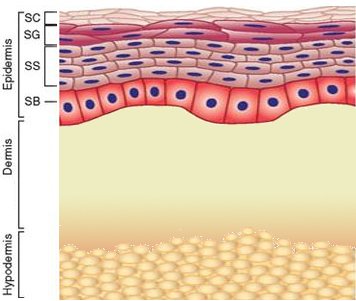
\includegraphics[width=0.5\textwidth]{figures/intro-skin_layers.jpg}
	\caption[Cross-section of layers of human skin]{\label{fig:intro-skin_layers}The three main layers of skin: The epidermis, the dermis, and the subcutaneous layers. Cells of the epidermis begin at the stratum basale (SB) and migrate through the stratum spinosum (SS) and stratum gradulosum (SG) to the stratum corneum (SC). Modified with permission: \textcopyright David J. Wong (\url{http://www.stembook.org}), \href{http://creativecommons.org/licenses/by-sa/3.0/}{CC-BY-SA-3.0}.\cite{Wong2009}}
\end{figure}

The second layer of skin is the dermis. It contains mostly collagen and elastin fibers but is also the location of capillaries and some nerves. The average dermal thickness is approximately 1.5 mm but can vary widely depending on the site.

Below the skin is the subcutaneous layer, also known as the hypodermis or subcutis. The thickness of this layer varies greatly because this is the layer that contains subcutaneous fat. This is also the location of the majority of superficial veins which can occasionally be visible at the surface. A representative thickness for this layer is 5 mm.

Light in the visible spectrum (400-750 nm) is only able to penetrate the first two layers of skin.\cite{Kochevar2012a} For 500 nm light (green/blue), the average penetration depth in human skin is 0.6 mm while for 700 nm light (red/near-infrared), the average depth is 1.2 mm. Diffusely reflected light must first travel into and then out of the skin, therefore the majority of the reflected light signal is due to scattering and absorption events within the epidermis and dermis. Within these layers, the dominant chromophores are: oxy- and deoxy-hemoglobin, and melanin. The relative absorption coefficients for these three chromophores is shown in Figure~\ref{fig:intro-skin_chromophores}. While water does account for roughly 70\% (w/w) of human tissue,\cite{Nakagawa2010} its absorption below 700 nm is negligible. Similarly, beta-carotene (in the epidermis) and bilirubin (in the dermis) do not contribute at wavelengths above 450 nm. They are also found in relatively small concentrations in healthy human skin. Although it contribution is small, there is a significant amount of absorption by the structural components of skin.\cite{Bargo2005}

\begin{figure}
	\centering 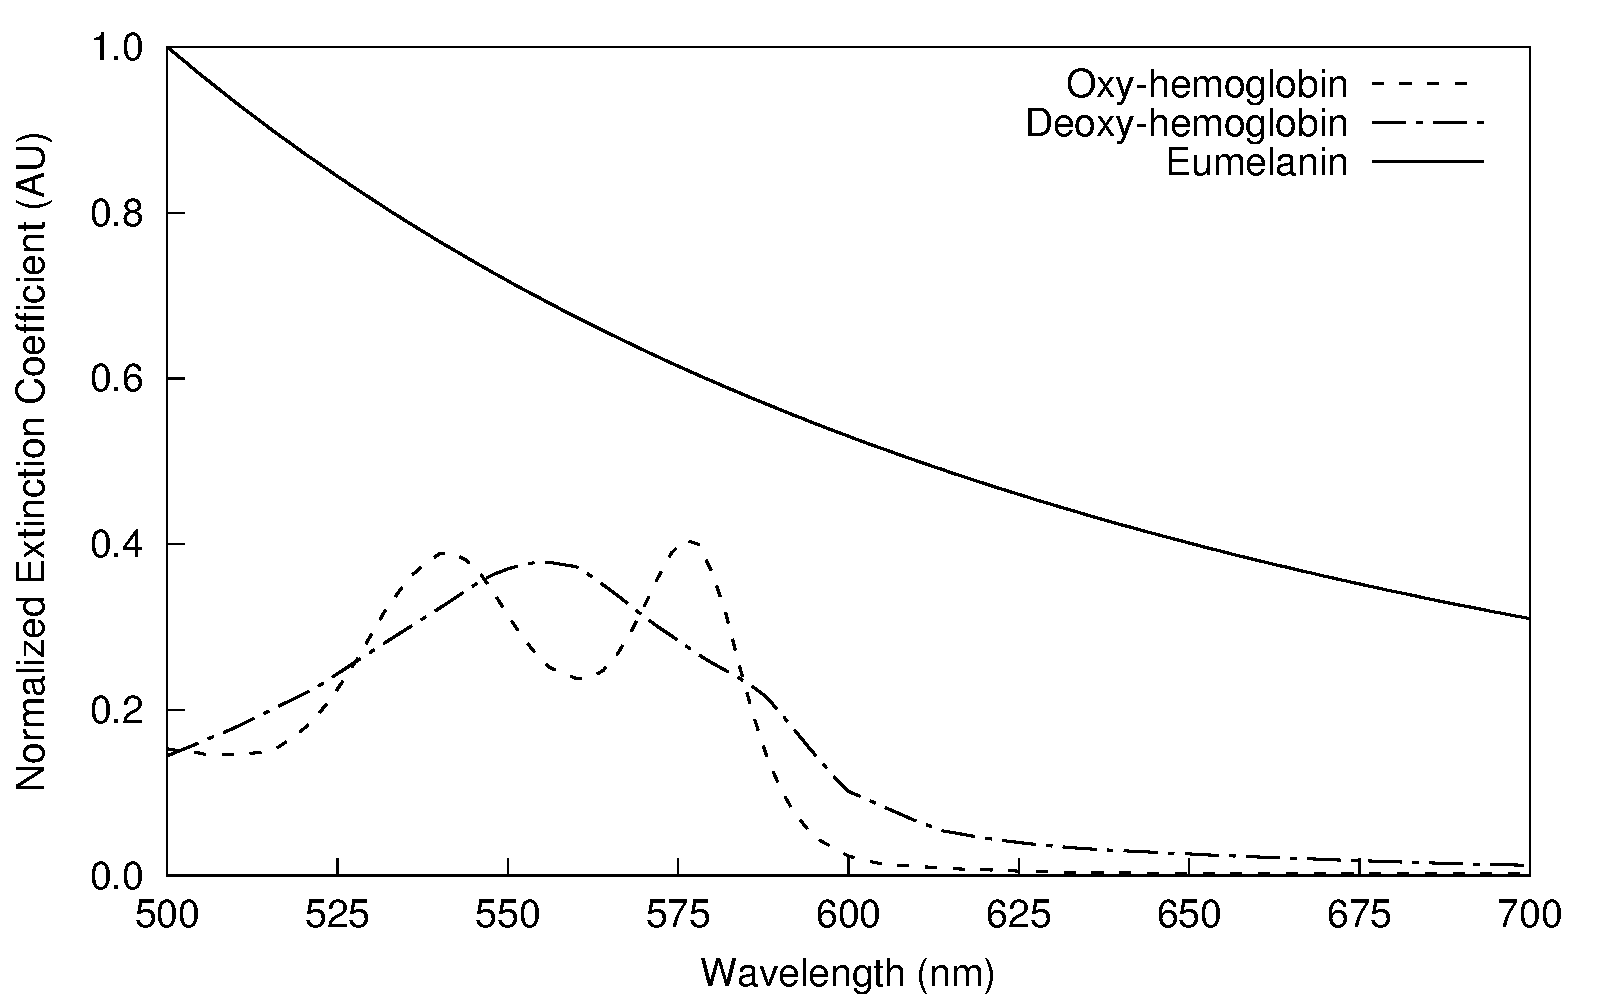
\includegraphics[width=0.8\textwidth]{figures/intro-skin_chromophores.png}
	\caption[The major chromophores of skin within the visible light spectrum]{\label{fig:intro-skin_chromophores}The major chromophores found in skin within the visible light spectrum are oxy- and deoxy-hemoglobin and melanin. Data shown are from Prahl \& Jacques (2001).\cite{Prahl2001}}
\end{figure}

\subsection{Physiology}
Perfusion is the process of delivering blood to capillaries, such as those in the dermal layer of the skin. Changes to the vasculature impact the blood flow within the skin that, in turn, changes the physical appearance at the surface. When the blood vessels narrow, less blood is present in the dermal layer of the skin. This process is known as vasoconstriction and results in a perceived blanching of the skin. When the blood vessels expand in a process known as vasodilation, more blood is present in the skin, which appears redder to the human eye.

It is important to note that, as illustrated in Figure~\ref{fig:intro-skin_chromophores}, both oxy- and deoxy-hemoglobin have low absorption in the red region of the visible spectrum, but have significant absorption within the green/yellow region. Therefore, when vasodilation occurs, the skin does not appear redder because more red light is being reflected. Rather, it is because less of the other colors are reflected. Similarly, when vasoconstriction occurs, more green and yellow light is reflected, contributing to a whiter appearance as white light is a collection of all of the colors within the visible spectrum. In regards to the ratio of the two hemoglobin chormophores during these two processes, McNaulty \emph{et al.} determined that the tissue oxygen saturation ($StO_2$) is related to blood flow.\cite{McNulty2011} Therefore, more oxy-hemoglobin is present during vasodilation and less is present during vasoconstriction.

Vasoconstriction and vasodilation are normal thermal regulatory responses of the human body.\cite{Kellogg2012} When the body begins to overheat, blood vessels near the surface expand to release heat. When the body temperature drops, blood vessels in the skin constrict to maintain more blood flow in the core, thereby preserving heat within the body. While this is the most commonly observed cause of these two processes, both can be induced by other means. As previously mentioned, the anesthetic lidocaine acts as a vasodilator and epinephrine, a hormone, behaves as a vasoconstrictor. They are often used together in a subcutaneous injection to simultaneously numb the region of interest while keeping it blanched for better viewing and minimal bleeding during surgery. As the name suggests, the needle is inserted into the subcutaneous tissue below the dermis and acts on the blood vessels that span both layers. The actual volume impacted depends on the volume and concentration of the two injected drugs and can last up to several hours.

Vasodilation is also the most common response to inflammation because the increased blood flow supplies the affected tissue with more oxygen and white blood cells, which are useful when infection is involved. During radiation therapy, radiation dermatitis/erythema, occurs because some of the healthy cells in the basal layer are prevented from dividing.\cite{Fitzgerald2008} This disrupts the steady rate of progression of cells to the skin surface, causing an inflammatory response. Erythema is also promoted by an increase in skin dryness due to the destruction of sweat and oil (sebaceous) glands. Although all patients respond differently and are prescribed different treatment plans, the general trend is for erythema to appear around the second week of treatment and can last for two to four weeks after treatment. For head and neck intensity modulated radiation therapy (IMRT), anecdotal evidence predicts that the maximal skin response will occur during the fifth week of treatment.

\section{Thesis proposal}
Currently available commercial systems for monitoring erythema rely on total diffuse reflectance spectroscopy. As a result, they can only provide measurements in the form of a skin reddness scale (or ``erythema index''). Such an index is only capable of detecting when skin is more or less red compared to some baseline measurement, and it cannot account for changes in non-hemoglobin chromophores.

Other clinical systems rely on a spatially-fixed spectrally-constrained diffuse reflectance approach. Such systems are capable of accounting for changes in the non-hemoglobin chromopores but are difficult to use and are sensitive to positioning errors.

A combination of the two approaches will result in a user-friendly system capable of accounting for all chromophore concentration changes. Thus, a spectrally-constrained model to interpret the total diffuse reflectance spectra obtained with an integrating sphere is proposed. In Chapter~2, a paper is presented that outlines the elements of such a system and how its response should be characterized. In Chapter~3, the system, combined with a standard erythema index, was used to determine the time to maximal effect of epinephrine. In Chapter~4, a paper proposing a spectrally-constrained model for interpreting the spectra obtained with the established system is presented. Special consideration is paid to the necessary corrections required when the total diffuse reflectance spectrum is collected instead of the standard fixed-position diffuse reflectance spectrum. The system and model are then combined in Chapter~5 and used to monitor the skin redness of patients undergoing IMRT for cancers of the head and neck. The results are used to outline the proper implementation of quantitative analysis in a study comparing two treatment interventions or management regimens. Such additional consideration is necessary due to the large daily variation in the hemoglobin concentration in skin. Along with the skin redness measurements, weekly TLD readings were performed to confirm the skin dose in the measurement region. This data was later deemed to have its own intrinsic value, and was used to determine TLD placement and positioning reproducibility in Chapter~6.
%\printbibliography{}
\printbibliography[heading=subbibliography]

\chapter{Paper I - The total diffuse reflectance spectroscopy system}
\section{Preamble}
text

\section{Contents}

\begin{center}

\textbf{Inexpensive diffuse reflectance spectroscopy system for measuring changes in tissue optical properties}

\bigskip
\bigskip

Diana L. Glennie, Joseph E. Hayward, Daniel E. McKee, and Thomas J. Farrell

\bigskip
\bigskip

\textit{Department of Medical Physics and Applied Radiation Sciences, McMaster University, 1280 Main Street West, Hamilton, Ontario, L8S 1A8}

\textit{AND}

\textit{Department of Medical Physics, Juravinski Cancer Centre, 699 Concession Street, Hamilton, Ontario, L8V 5C2}

\end{center}

\bigskip
\bigskip

\noindent Journal of Biomedical Optics (Oct 07, 2014).

\noindent http://dx.doi.org/10.1117/1.JBO.19.10.105005

\subsection{Introduction}
The ability to quantify changes in the concentration of chromophores in the skin (particularly oxy- and deoxy-hemoglobin) in vivo and in real time has many applications in healthcare. For example, a complication of radiation therapy is radiation-induced erythema, which, if not monitored closely, can progress to painful moist desquamation.\cite{Hopewell1990,Russell1994,Nystrom2004,Fitzgerald2008} In photodynamic therapy, tissue oxygenation can be used to indicate treatment efficacy\cite{Woodhams2007} since oxygen is required for the activation of the cytotoxic photochemicals.\cite{Patterson1989a,Wilson2008} Finally, in plastic surgery, proper blood flow is integral for the success of free tissue transplants and is used to indicate whether or not a return to the operating room is necessary.\cite{Steele2011}

Several methods have been validated for measuring skin redness. In increasing complexity and accuracy they are visual assessment (with or without a color chart), colorimetry/photography, and spectroscopy.\cite{Agache2004} Although the visual assessment technique,\cite{Trotti2003} is the most common, it is qualitative in nature. Due to its subjective nature and the nonlinearity of human vision, it is highly prone to interobserver as well as intraobserver variations.\cite{Bodekaer2013} The subjectivity of this method can be minimized by the introduction of color charts; however, a very large number of color shades would be required to best account for the effect of pigmentation on the perceived redness. Despite these difficulties, visual assessment remains the gold standard for measuring skin redness.\cite{Basketter1997,Wengstrom2004}

Digital photography is usually approached as a two-dimensional implementation of colorimetry. In colorimetry, the color is quantified using a set of three specifically tuned color sensors (usually RGB) that represent the color using a standard color map, such as the L*a*b* system from the International Commission on Illumination (CIE).\cite{CI2012} Colorimetry (and digital photography) is made extremely difficult by the necessity to calibrate and standardize the results to allow for intermeasurement comparison (between days or between individuals).\cite{Jung2012} Following correct calibration, both methods are capable of detecting changes in blood and oxygen saturation but, since the relationship between the measured data and skin redness is not fully characterized, they are only capable of indicating whether the skin is more or less red in comparison to previous or baseline measurements.\cite{Kollias2002,Canning2009,Nishidate2011,Setaro2002}

Spectroscopy-based methods, such as reflectance spectroscopy and hyperspectral imaging, are the most complex of the methods used for measuring skin color.\cite{Zhang2005,Stamatas2008,Kollias2010,Yudovsky2010,Chin2012} Spectroscopy provides quantitative data across a range of wavelengths, allowing for different parameters to be extracted from its measurements, depending on the scope of the investigation and the apparatus used. User-friendly commercial models capable of monitoring relative erythema and tissue oxygen saturation are expensive and use single-use detection probes. For example, the T-Stat\textregistered (Spectros, Portola Valley, California) costs approximately \$25,000 US.\cite{Fox2012} Cheaper models are less user-friendly and mostly only provide a single value for oxygen saturation. As a result, these systems are primarily used by highly trained investigators at research institutions and are rarely utilized in a typical clinical setting where they could be used routinely and would prove most beneficial.

In order to facilitate the translation of spectroscopy systems from the research laboratory to the routine clinical setting for the use on human skin in vivo, an economic integrating sphere-based diffuse reflectance spectroscopy (DRS) unit was developed and characterized. The system designs and specifications will be outlined. To illustrate the validity and utility of the assembled system, the results of two ongoing clinical studies measuring erythema under different conditions will be presented.

\subsection{Design of the Total DRS System}
Simply, the total DRS system consists of a white light source coupled to an integrating sphere via an optical fiber. A second detection optical fiber directs the reflected light to a spectrometer. The spectrometer is controlled by a computer on which the required processing software was installed. A schematic of the system design is shown in Figure~\ref{fig:p1-sys_diagram}. A detailed description of the selection of each component is presented below.

\begin{figure}
	\centering 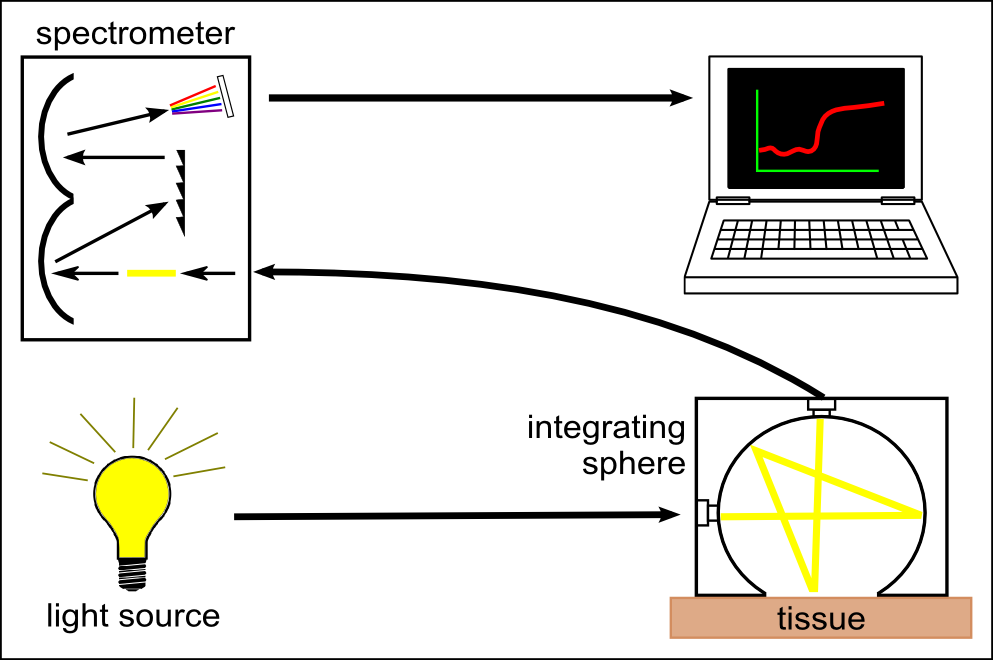
\includegraphics[width=0.6\textwidth]{figures/p1-sys_diagram.png}
	\caption[System schematic]{\label{fig:p1-sys_diagram}A schematic of the measurement system (not to scale). The light source is connected to the side port of the integrating sphere. Light collected through the overhead port is detected by the spectrometer and processed by the laptop.}
\end{figure}

\subsubsection{Light Source}
Oxy- and deoxy-hemoglobin have spectral absorption features within the visible light range.\cite{Young1997,Lister2012} Therefore, a light source encompassing this range, without any narrow bandwidth spectral excitation features, is required. In addition, a stable output over the measurement period (minutes to hours) is required for proper reflectance calculation. An Oriel 77501 Radiometric Fiber Optic Source (Newport, Irvine, California) was chosen with a 100 W quartz tungsten halogen lamp to produce a highly stable output within the visible-NIR wavelength range that can be easily coupled to an optical fiber. It also has an adjustable iris to allow for output optimization.

\subsubsection{Spectrometer and Optical Fibers}
The spectrometer must be capable of detecting light with high sensitivity across the visible spectrum. It must also have sufficient spectral resolution to allow for the differentiation between the spectral features of oxy- and deoxy-hemoglobin (<13 nm for oxy-hemoglobin). An ideal spectrometer would also be small for ease of portability.

The S2000 Miniature Fiber Optic Spectrometer from Ocean Optics (Dunedin, Florida) was chosen for this system. It has a wavelength range of 340 to 1000 nm and a dynamic range of 2000 for a single scan. The 2048-element linear CCD-array results in a pixel width of approximately 0.35 nm and the integration time can range from 3 ms to 60 s. Its small size (<150 mm cube) allows for easy transportation between clinical sites.

The fiber optic connector specifications for the Ocean Optics spectrometer are for an SMA 905 to single-strand 0.22 NA optical fiber. The optical fiber acts in place of a slit in the spectrometer’s hardware. A relatively large fiber core of 400 \si{\um} was chosen to maximize light collection. This resulted in spectral resolution of 10 nm as determined from the measurement of a mercury–argon calibration source (HG-1 Mercury Argon Calibration Source, Ocean Optics, Dunedin, Florida). The effect of this spectral resolution on the reflectance spectrum analysis is described in Section~\ref{sec:ei_analysis}. The final criterion for the fibers was high transmission in the visible spectrum. Two such fibers, with a wavelength range between 400 and 2200 nm, were purchased from Thorlabs (Newton, New Jersey).

\subsubsection{Integrating Sphere}
The size of the integrating sphere is dictated by its use to measure light reflectance from human skin. As such, the integrating sphere should be relatively small (on the order of 5 to 10 cm in diameter) so that it can fit onto the various curves of the human body. A small sphere would also be easier to maneuver and keep stationary, resulting in more stable measurements.

The size of the measurement port of the sphere should be sufficiently large that local inhomogeneities in the measurement area (such as small freckles or hairs) do not overwhelm the result, but should result in the sphere’s port fraction (the ratio of the total port area to the total internal surface area of the sphere) falling between 2\% and 5\%.\cite{Hanssen2002} For the range of sphere sizes suggested above, the port diameter would fall somewhere within 1.5 to 5 cm.

The sphere should also have a high internal reflectance (greater than 94\%) and produce a uniform light field at the measurement port.\cite{Labsphereb,Labspherea,Labsphere} If the input light is directly incident on the detection port, the sphere should include a baffle, blocking this path. For spheres of the size used in this experiment, baffles should be avoided when possible as they disrupt the internal surface of the sphere, reducing the uniformity of the illumination within the sphere.

The integrating sphere was made from a cube of Spectralon\textregistered (Labsphere\textregistered, North Sutton, New Hampshire) with side lengths of 2 in. (50.8 mm). The cube was bisected and a hemispherical cavity was machined into both halves using a 1\textonequarter in. (31.75 mm) ball-end mill. The bottom of one of these halves was milled down, creating a port measuring 15.2 mm in diameter. The parts were assembled to form the sphere and holes were drilled through the center of the unmilled half as well as through one side at the junction to accommodate SMA 905 connectors which would become the detection and illumination ports, respectively (see Figure~\ref{fig:p1-intsphere_schematic}).

\begin{figure}
	\centering 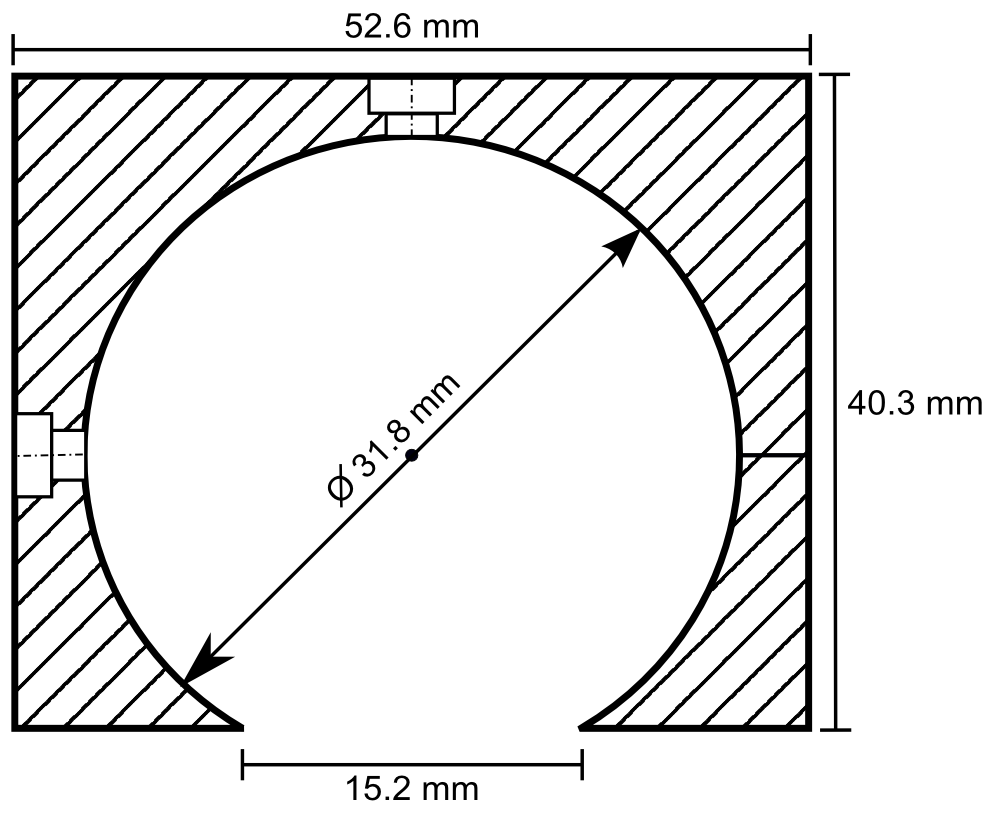
\includegraphics[width=0.5\textwidth]{figures/p1-intsphere_schematic.png}
	\caption[Cross-sectional diagram of the integrating sphere]{\label{fig:p1-intsphere_schematic}A cross-sectional diagram of the integrating sphere. The block of Spectralon\textregistered used to make the sphere is bisected before processing and then reattached to form the sphere.}
\end{figure}

\subsubsection{Implementation Costs}
The specifications for each individual component have some flexibility; therefore, a DRS system can be built within a wide range of costs while still achieving the same measurement results.

In choosing the light source, it is only important that it covers the desired wavelength range and be stable to within 1\%. Although a uniform spectral output is ideal to keep the signal uncertainty relatively constant, it is not necessary. A quartz tungsten halogen lamp provides smooth spectral features and high output powers; however, a less expensive alternative would be a white LED. These provide excellent illumination and are relatively stable, although they do have an emission peak in the blue region (\textasciitilde465 nm).

Integrating spheres can be purchased from an optical device supplier; however, spheres can be built for costs as low as \$100 US by obtaining a suitable block of Spectralon. Since the sphere is not being used for radiometric purposes, it can deviate from an ideal integrating sphere and still provide an accurate reflectance measurement. Spheres can also be constructed by vacuum-forming plastic styrene about a spherical mold and coating the inside with barium sulfate paint.\cite{Glennie2009}

The most expensive piece of equipment component is the spectrometer, and its price will depend on the detection sensitivity and grating size. The average cost for a common fiber-based spectrometer is around \$2000 US. Although not recommended, spectrometers can also be built cheaply if necessary.\cite{Sumriddetchkajorn2012}

The computer must be able to interface with the spectrometer and run the necessary software. Therefore, an inexpensive netbook or laptop will be sufficient. Optical fibers are uniformly priced in the market and will contribute very little to the total cost of the system.

A list of itemized expenses is shown in Table 1, assuming new materials were required. For comparison, a hand-held colorimeter is available for \$6000 US from Derma Spectrometer (MIC Global, London, United Kingdom).

\begin{table}[h]
	\centering
	\caption{Cost estimates for the DRS system. Listed prices are based on the purchase of new material.}
	\label{my-label}
	\begin{tabular}{lcc}
		\toprule
		\multirow{2}{*}{Component} & \multicolumn{2}{c}{Pricing (USD)} \\ \cmidrule(l){2-3} 
		& Low             & High            \\ \midrule
		Light source               & \$100           & \$500           \\
		Integrating sphere\qquad\qquad         & \$100           & \$1500          \\
		Spectrometer               & \$500           & \$3000          \\
		Computer                   & \$250           & \$500           \\
		Connection cables\qquad\qquad          & \$100           & \$200           \\
		\textbf{Total}             & \textbf{\qquad\$1050\qquad} & \textbf{\qquad\$5700\qquad} \\ \bottomrule
	\end{tabular}
\end{table}

\subsection{Procedure and Performance}

\subsubsection{Integrating Sphere Configuration}
The optical fibers are connected to the integrating sphere following a d/0\degree (diffuse illumination/direct detection) geometry such that the input light is first incident on the sphere wall before encountering the tissue surface and the output fiber is directly across from the measurement port (as shown in Figure~\ref{fig:p1-sys_diagram}. In this geometry, the sample is more uniformly illuminated compared with a 0\degree/d geometry due to the multiple reflections of the light prior to exiting the sphere at the tissue. In addition, since the illumination is diffuse rather than normally incident, the penetration of light is more superficial due to the oblique entrance angle (average 55\degree). Thus, a greater percentage of spectroscopic information originates from the upper layers of skin where the chromophores of interest are located. Due to the small size of this integrating sphere, a baffle was not used. The geometry and the detector fiber acceptance angle (0.22 NA) allowed only light that was specularly or diffusely reflected from the tissue surface to be collected.

\subsubsection{Calculating Spectral Reflectance}
The spectral reflectance of a tissue sample was normalized by dividing the spectral count rate with the detection port on the tissue, $S_t(\lambda)$, by the spectral count rate from a highly reflecting standard, $S_{norm}(\lambda)$. Both of these were adjusted by subtracting the background signal rate, $S_{bg}(\lambda)$, so that the modified total diffuse reflectance, R*m(?), is given by

\begin{equation}
	R_m^\ast(\lambda)=\frac{S_t(\lambda)-S_{bg}(\lambda)}{S_{norm}(\lambda)-S_{bg}(\lambda)}.
\end{equation}

Normalizing to a reflectance standard eliminates the need to correct the measured signal rate for the system spectral response.

A 99\% reflectance standard (SRS-99-010, Labsphere, North Sutton, New Hampshire) was used as the normalization standard while a 2\% reflectance standard (SRS-02-010, Labsphere, North Sutton, New Hampshire) was used for the background. The 2\% standard was used instead of directing the detection port into a dark room in order to avoid changes in ambient lighting conditions, should the system be used in different locations which would affect the calculated reflectance. This substitution did not affect the accuracy or precision of the measurement. If reflectance standards are not available, a piece of thick, matte black cloth may be substituted for the 2\% standard, and a piece of high diffusely reflective material such as a piece of Spectralon or a flat surface coated with barium sulfate may be substituted.

For each spectral count rate measurement, the integration time was set such that the maximum intensity was approximately 90\% of the dynamic range. This allowed for optimal precision while ensuring that the signal would not saturate. Five measurements were averaged to further reduce the noise. The averaged measurements were converted into a count rate by dividing by the integration times.

\subsubsection{Sphere Preparation}
The measurement port of the integrating sphere was covered with a sheet of occlusive dressing (Tegaderm\texttrademark film, 3M Health Care, St. Paul, Minnesota) in order to prevent dirt and other material from contaminating the inside of the sphere. A new sheet was applied for each patient before any measurements to ensure sterility. The dressing was left on for the normalization and background measurements and, therefore, did not modify the resulting reflectance. Reflectance measurements were performed on calibrated diffuse reflectance standards ranging from 2\% to 99\% (RSS-08-010, Labsphere, North Sutton, New Hampshire) with the dressing in place and removed. Both sets of measurements showed no measurable difference.

\subsubsection{Correcting for Single Beam Substitution Error}
Single beam integrating spheres used for reflectance spectroscopy suffer from single beam substitution error\cite{Springsteen1998,Labspherec} due to the decrease of the total flux within the sphere when the normalization plate is replaced with the sample. This can be corrected using Equation~\ref{eq:sbse}. The parameters (a, b, c), as a function of wavelength, were determined empirically by measuring the calibrated reflectance standards described in the previous section and developing a relationship between the measured and calibrated reflectances (represented by $R_m^\ast$ and $R_m$, respectively), based on the fraction of reflected light. If reflectance standards are not available, Intralipid\texttrademark (Baxter, Deerfield, Illinois) and India ink liquid phantoms can be used as they have well-characterized extinction coefficients.\cite{Flock1992,Madsen1992}

\begin{equation}
\label{eq:sbse}
	R_m = \frac{aR_m^\ast + b}{R_m^\ast + c}
\end{equation}

These data were fit using a nonlinear least-squares algorithm at each of the wavelengths. A typical fit for a single wavelength is shown in Figure~\ref{fig:p1-sbse_cf}. This correction was applied to the modified total diffuse reflectance, resulting in a corrected total diffuse reflectance ($R_m$). A set of colored diffuse reflectance standards (CSS-04-010, Labsphere, North Sutton, New Hampshire) were measured and, following correction, the measured reflectance was within 0.01 of the calibrated reflectance specified by the supplier (Figure~\ref{fig:p1-colored_refl}).

\begin{figure}
	\centering 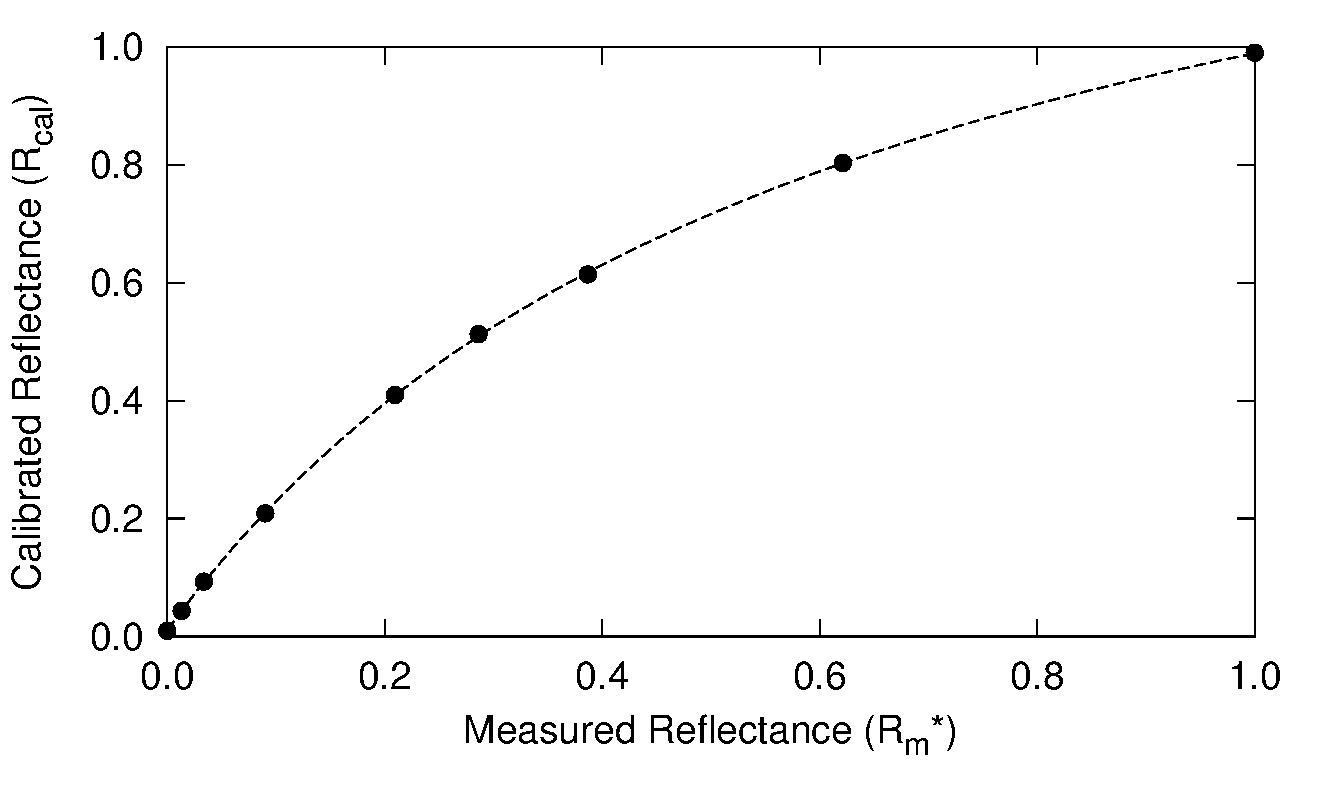
\includegraphics[width=0.7\textwidth]{figures/p1-sbse_cf.png}
	\caption[Single-beam substitution error correction curve text]{\label{fig:p1-sbse_cf}The integrating sphere calibration curve at 600 nm. The fitted function corrects the measured reflectance for single-beam substitution error. The dots are the calibrated and measured reflectance pairs and the dashed line is the fit to these data.}
\end{figure}

\begin{figure}
	\centering 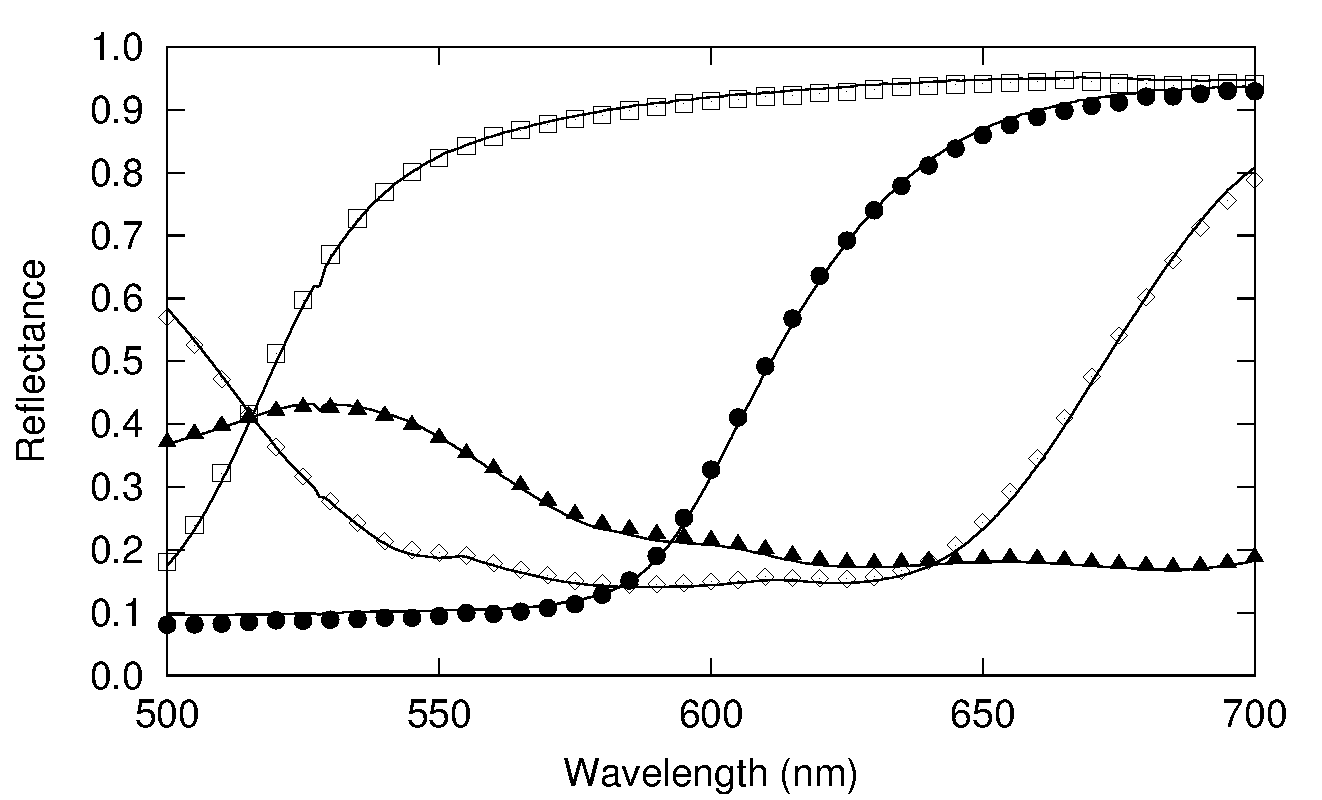
\includegraphics[width=0.7\textwidth]{figures/p1-colored_refl.png}
	\caption[Measured and calibrated reflectance spectra]{\label{fig:p1-colored_refl}The measured (symbols) and calibrated (lines) reflectance spectra for a set of four colored diffuse reflectance standards: red (CIRCLE), yellow ($\square$), green (TRIANGLE), and blue ($\diamond$). Correction for the single-beam substitution error brought the measured reflectance values to within 0.01 of the calibrated reflectance specified by the supplier.}
\end{figure}

\subsubsection{Reflectance Measurement Reproducibility}
The reproducibility of the system was tested using the green reflectance standard (SCS-GN-010) because it had reflectance similar to human skin and spectral features in the same region as hemoglobin. Reflectance was measured every day for 30 days and the standard deviation across the 500 to 700 nm spectral region never exceeded 1\%. As expected, it varied with the spectral reflectance of the reflectance standard (i.e., the uncertainty was lower when the reflectance/signal was higher). Reproducibility measurements were also performed on human skin and they had a similar result.

\subsection{Experimental Validation}

\subsubsection{Study Overviews}
In order to demonstrate the use and validity of the DRS system, sample data from two ongoing erythema studies are presented. In the first study, erythema and skin blanching were induced via subcutaneous injection of lidocaine (a vasodilator and anesthetic) with or without epinephrine (a vasoconstrictor) over the deltoid muscles of volunteers’ upper arms. The aim of this study was to determine the time to maximal effect of injected epinephrine. In the second study, serial skin reflectance measurements were taken on head and neck cancer patients undergoing intensity-modulated radiation therapy (IMRT). The goal of this study was earlier detection of radiation-induced erythema compared with visual assessment methods. Both studies received Hamilton Health Sciences Research Ethics approval.

\subsubsection{Erythema Index Analysis}
\label{sec:ei_analysis}
The measured reflectance spectra were processed using the Dawson erythema index (EI).\cite{Dawson1980} This model was chosen because of its wide acceptance and use (over 280 citations to date),\cite{Riordan2001} as well as its straight-forward calculation method. Briefly, the EI is the area under the curve of the log of the inverse reflectance spectrum between 510 and 610 nm (encompassing the absorption features of oxy- and deoxy-hemoglobin). The influence of melanin in the EI can be approximately corrected using reflectance data between 650 and 700 nm (EI). For serial measurements on an individual, a relative erythema index (EI\textsubscript{r}) can also be calculated. Simply, a baseline EI\textsubscript{c} is obtained either at time zero or at a nearby reference location. This is subtracted from EI\textsubscript{c} values measured at later time points such that, in the absence of changes in hemoglobin, EI\textsubscript{r} would be zero.

The 10 nm FWHM spectral resolution of the system has the effect of broadening spectral features in the measured reflectance. Although this would be problematic for narrow features, the absorption features in the hemoglobin spectra are very broad and were not strongly affected. To verify the effect on the EI, spectra derived from the literature\cite{Jacques1998} were convolved with a 10 nm FWHM Gaussian function and the EI calculated before and after. Small differences in the calculated EI were noted (data not shown), however changes in EI with respect to an increase or decrease in hemoglobin were insensitive to the spectrometer’s spectral resolution.

\subsubsection{Study Results}
In the first study, the reflectance was measured serially for 2 h following the injection of lidocaine (with or without epinephrine) and the measurements were processed to calculate the EIr as a function of time. A time course for one volunteer is shown in Figure~\ref{fig:p1-lido_epi} along with the reflectance spectra at specific time points. For both injections, there was a rapid increase in the EI\textsubscript{r} indicating an increase in the hemoglobin content. The combined lidocaine and epinephrine injection then decreased to a minimum EI\textsubscript{r} of approximately -16 at the 22 min mark indicating a reduction in hemoglobin content. An analysis of the EI\textsubscript{r} for all subjects indicated that the maximum epinephrine-induced blanching occurred approximately 25 min following injection, after which surgical incision may commence.\cite{McKee2013}

\begin{figure}
	\centering 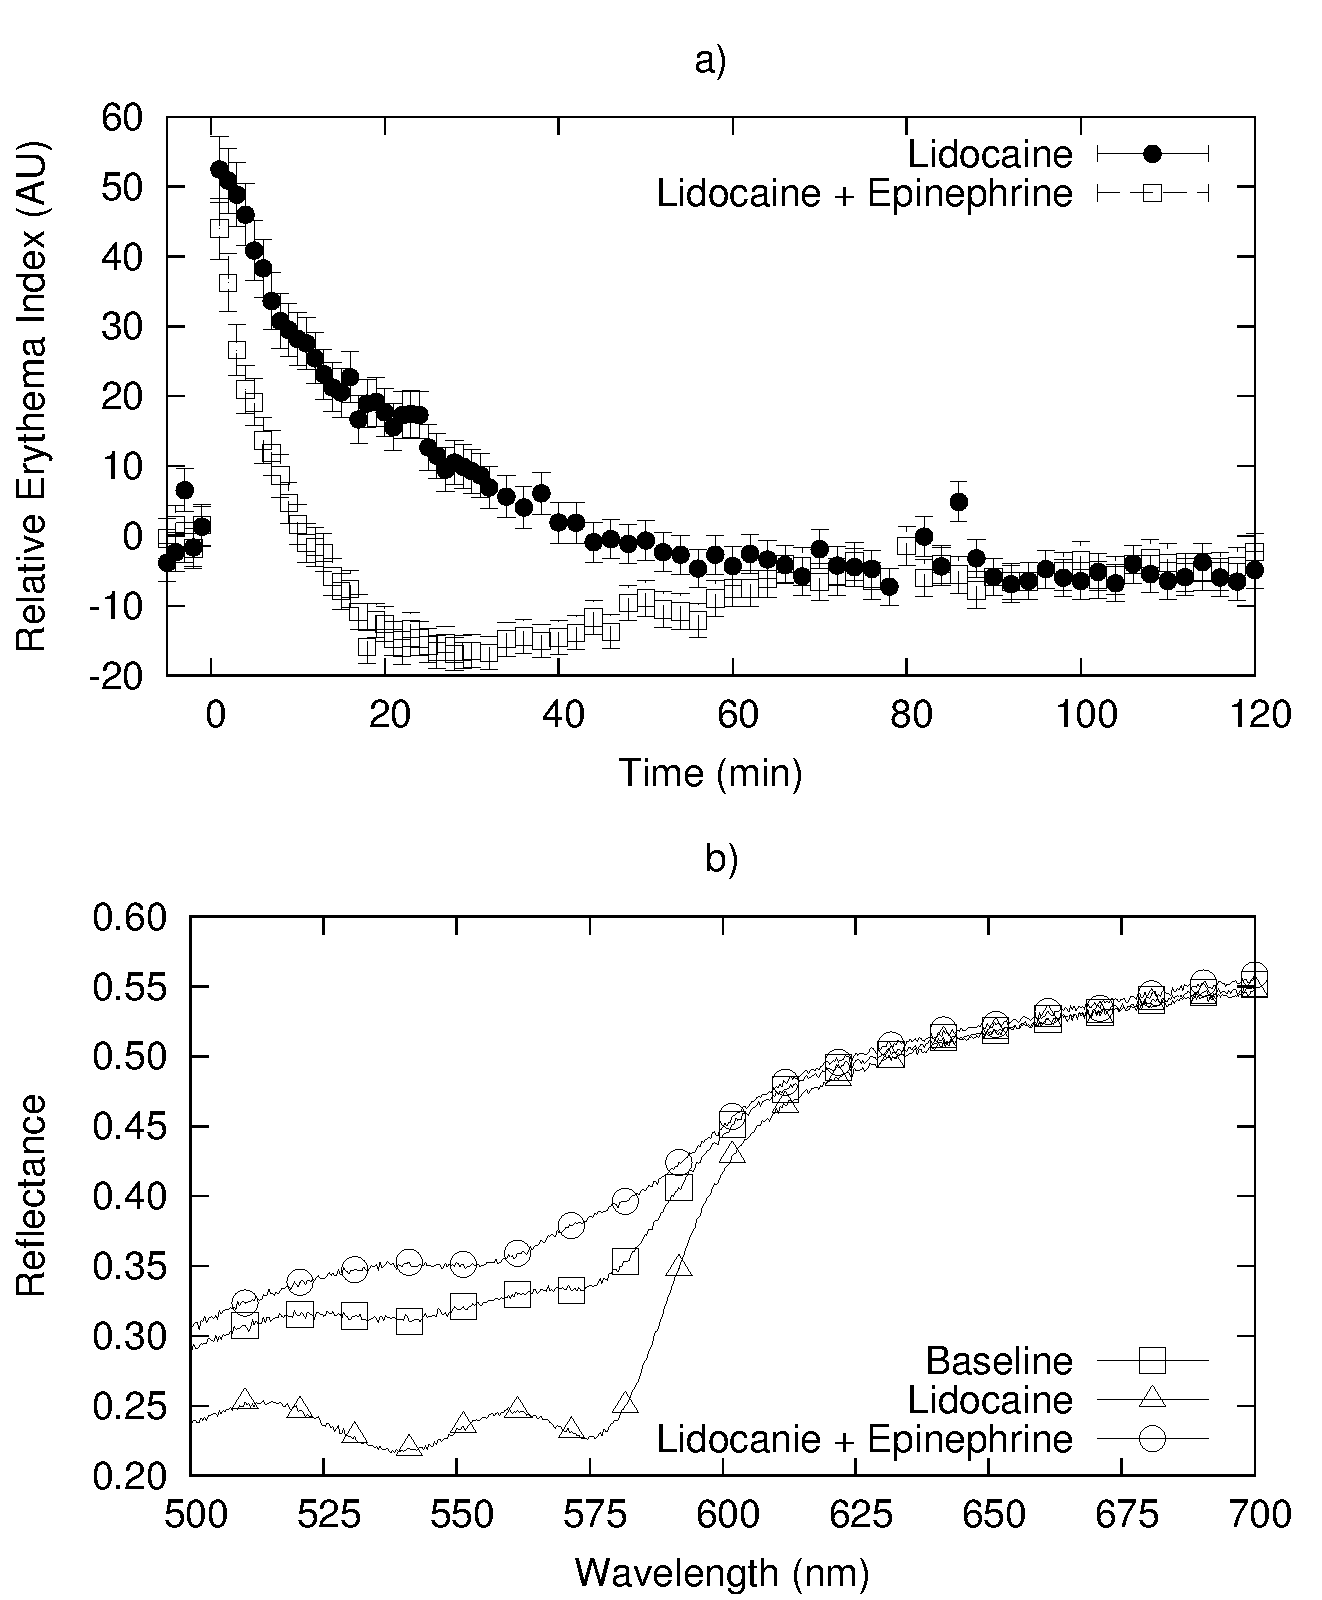
\includegraphics[width=0.7\textwidth]{figures/p1-lido_epi.png}
	\caption[Sample time course for lidocaine \& epinephrine]{\label{fig:p1-lido_epi}(a) A sample time course for one volunteer in the study involving lidocaine and epinephrine. (b) Full reflectance spectra from before injection ($\square$), 1 min following the injection of lidocaine alone ($\triangle$), and 26 min following the injection of lidocaine and epinephrine ($\bigcirc$).}
\end{figure}

In the second study, the reflectance was measured daily over the course of the patients’ head and neck IMRT treatments. During this study, it was necessary to have multiple investigators operate the DRS system. This requirement illustrated the ease of training associated with the system, as all investigators were capable of properly using the system following a short 15 min tutorial. Greater variation was observed in the daily measurements compared with the short-term measurements of the first study (see Figure~). The EI\textsubscript{r} was not calculated because the baseline consisted of a single measurement. The variation is the result of daily changes such as time of day and patient temperature.\cite{Fullerton1996} An increase in EI\textsubscript{c} was observed over the course of the 35 days. Erythema was first visually diagnosed on day 18 of treatment. This study is ongoing.

\begin{figure}
	\centering 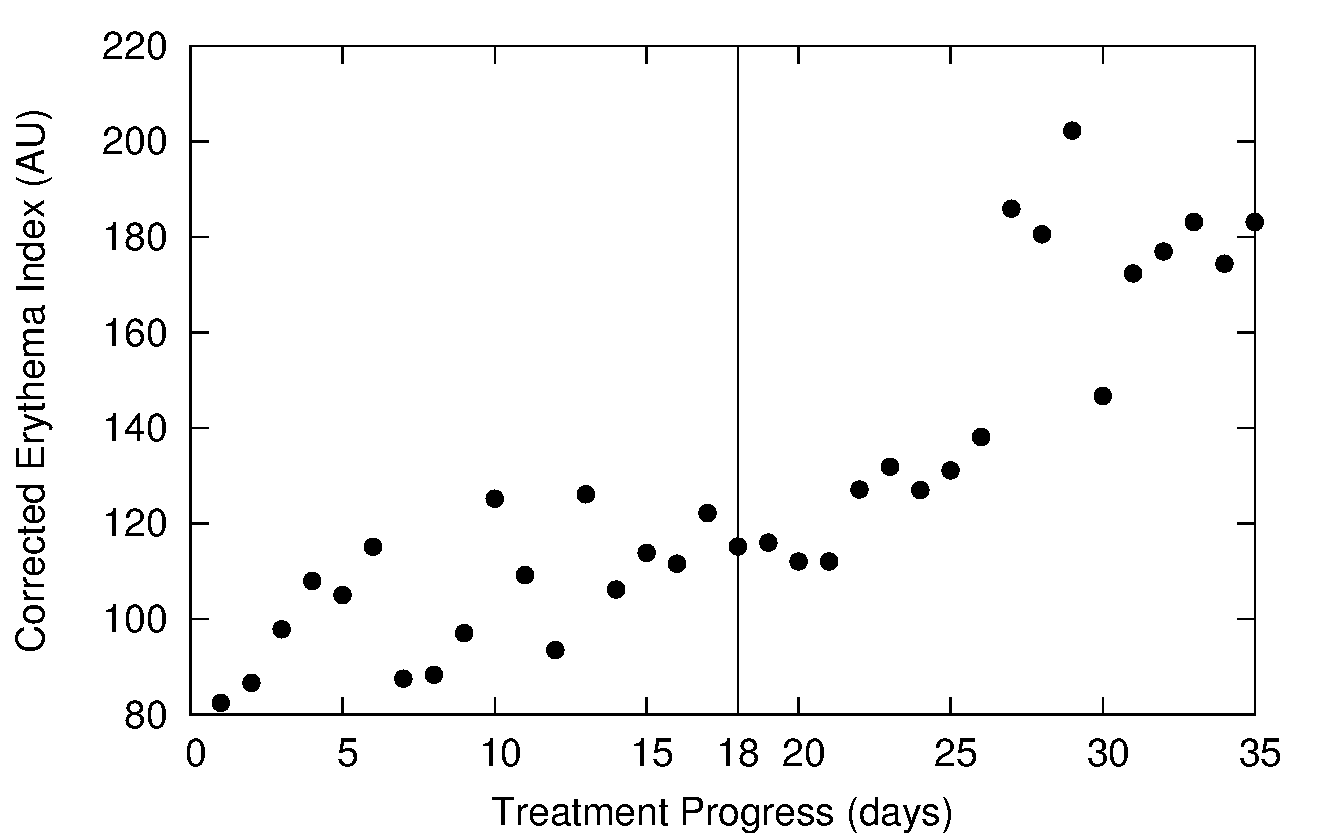
\includegraphics[width=0.7\textwidth]{figures/p1-cor_ei.png}
	\caption[Corrected erythema index for IMRT cancer patient]{\label{fig:p1-cor_ei}Corrected erythema index for a head and neck IMRT cancer patient. Daily measurements were taken over the course of treatment. Erythema was not visually noted until day 18.}
\end{figure}

\subsection{Discussion}
This paper illustrates two clinical applications of a DRS system. These results demonstrate that a low-cost spectroscopy system is capable of measuring spectral changes in reflectance due to changes in the concentration of hemoglobin. These changes were quantified using the Dawson EI. The system is easy to operate and yields valuable clinical data with little training required. The system described here may be found to have a wide range of clinical assessment roles, which would make it an even more useful tool for health care practitioners. However, since the system collects a full spectrum, it is capable of generating much more valuable information than just a single EI value. For example, correcting for background chromophores is only approximate and any changes over the measurement period could register as incorrect increases or decreases in skin redness. An alternative modeling approach using a spectrally constrained diffuse reflectance model to fit the measured reflectance spectrum with concentrations of the major tissue chromophores may be advantageous. This will allow for the detection of skin color changes in reference to their responsible chromophore, but would require the measured spectrum to be extremely accurate and precise.

One of the limitations of this spectroscopy system is that the signal is normalized using a highly scattering Spectralon\textregistered standard. In comparison, human skin is much less scattering and therefore the true reflectance is under-represented due to scattering losses. These scattering losses are not large but, since they vary with the tissue optical properties, they would need to be accounted for in a spectrally dependent model.

This paper presents a low-cost, user-friendly DRS system for measurement of changes in skin hemoglobin concentration. The performance of the system was characterized in terms of wavelength accuracy and measurement stability, uncertainty, and reproducibility. The validity and utility of the system were demonstrated through a skin reddening/blanching experiment and a radiation-induced erythema study, followed by analysis with a simple erythema model. Further uses of the system have yet to be investigated.

\subsection*{Acknowledgments}
The authors would like to thank Kevin R. Diamond and Gabriel A. Devenyi for their assistance in the preparation of this paper. This work was financially supported by the Natural Sciences and Engineering Research Council of Canada.
\printbibliography[heading=subbibliography]

\chapter{Paper II - Application of system in plastic surgery}
%\include{chapter3}

\chapter{Paper III - A model for analyzing system-measured spectra}
%\include{chapter4}

\chapter{Paper IV - Application of system and model in radiation therapy}
%\include{chapter5}

\chapter{Paper V - TLD reproducibility}
%\include{chapter6}

\chapter{Conclusions}
%\include{chapter7}

%\nomenclature{EXPL}{Example Definition of Abbreviation}%

%\printbibliography{}
%\printindex

\appendix
\chapter{Appendix A}
\end{document}
